\documentclass[conference]{IEEEtran}
%\synctex=1

\usepackage{times}
\usepackage{graphicx}
\usepackage{epsfig}
% \usepackage{url}
% \usepackage{hyperref}
\usepackage{hyperref}
\usepackage{xspace}\usepackage{float}
\usepackage{latexsym}
\usepackage{natbib}
\usepackage[usenames]{color}
\usepackage{multirow}
\usepackage{listings}
\usepackage{textcomp}

\bibpunct{[}{]}{,}{n}{}{}

\def\denseitems{
  \itemsep1pt plus1pt minus1pt
  \parsep0pt plus0pt
  \parskip0pt\topsep0pt}

%\setpapersize{USletter}
%\setmarginsrb{2.54cm}{2.54cm}{2.54cm}{1.5cm}{0pt}{0mm}{0pt}{8mm}
%\setcounter{secnumdepth}{3}

\newcommand{\ie}{\textit{i.e.,} }
\newcommand{\eg}{\textit{e.g.,} }

\newcommand\opt[1]{}
\newcommand\find[1]{}

\newcommand{\xxx}[1]{{\color{red}\bf #1}}
\newcommand{\todo}[1]{{\color{red}\bf \ \\\noindent TODO: #1}}
\newcommand{\note}[1]{{\color{red}\bf \ \\\noindent NOTE: #1}}

\def\denseitems{
  \itemsep1pt plus1pt minus1pt
  \parsep0pt plus0pt
  \parskip0pt
  \topsep0pt
}
\leftmargini 1em
%  \leftmarginii-1em
%  \leftmarginiii-1em
%  \leftmarginvi-1em

\newenvironment{myquote}
  {\baselineskip=\SingleLine \begin{quote}
    {\setlength{\leftmargin}{2\parindent}}}
  {\end{quote} \baselineskip=\DoubleLine \vspace*{-\SingleLine}}

\def\bfcaption#1{\caption[#1]{\bf #1}}

\def\argmax{\mathop{\rm arg\,max}}

\def\denseitems{
  \itemsep1pt plus1pt minus1pt
  \parsep0pt plus0pt
  \parskip0pt\topsep0pt}

\newcommand{\ls}[1]
   {\dimen0=\fontdimen6\the\font 
    \lineskip=#1\dimen0
    \advance\lineskip.5\fontdimen5\the\font
    \advance\lineskip-\dimen0
    \lineskiplimit=.9\lineskip
    \baselineskip=\lineskip
    \advance\baselineskip\dimen0
    \normallineskip\lineskip
    \normallineskiplimit\lineskiplimit
    \normalbaselineskip\baselineskip
    \ignorespaces
   }

\newcommand{\crunchlist}{
        \setlength{\itemsep}{-0.05in}
        \setlength{\partopsep}{0in}
        \setlength{\topsep}{0in}}

\def\sqzhuge{\vspace{-14pt}}
\def\sqztiny{\vspace{-6pt}}

\def\definition#1#2{
\begin{smalldescription}
\item[Definition:] \underline{#1}\\
#2\hfill~$\Box$
\end{smalldescription}
%\vspace*{-5mm}
}

\def\definition#1{
\begin{smalldescription}
\item[Definition:]
#1\hfill~$\Box$
\end{smalldescription}
}

\def\ind#1{{\it #1}\index{#1}}

%% Alternative to itemize
\newenvironment{smallitemize}{
   \setlength{\topsep}{0pt}
   \setlength{\partopsep}{0pt}
   \setlength{\parskip}{0pt}
   \begin{itemize}
   \setlength{\leftmargin}{.2in}
   \setlength{\parsep}{0pt}
   \setlength{\parskip}{0pt}
   \setlength{\itemsep}{0pt}}{\end{itemize}}

%% Alternative to enumerate
\newenvironment{smallenumerate}{
   \setlength{\topsep}{0pt}
   \setlength{\partopsep}{0pt}
   \setlength{\parskip}{0pt}
   \begin{enumerate}
   \setlength{\leftmargin}{.2in}
   \setlength{\parsep}{0pt}
   \setlength{\parskip}{0pt}
   \setlength{\itemsep}{0pt}}{\end{enumerate}}

%% Alternative to description
\newenvironment{smalldescription}{
   \setlength{\topsep}{0pt}
   \setlength{\partopsep}{0pt}
   \setlength{\parskip}{0pt}
   \begin{description}
   \setlength{\leftmargin}{.2in}
   \setlength{\parsep}{0pt}
   \setlength{\parskip}{0pt}
   \setlength{\itemsep}{0pt}}{\end{description}}

%\long\gdef\TabPerf#1#2{%
%  #1 & #2 \\ \hline
%}

%% The [gray]{0} gives rise to the black color. For other shades of
%% gray, increase the number.
%\long\gdef\TabHead#1#2{%
%\multicolumn{1}{|>{\columncolor[gray]{0}}c|}{\textcolor{white}{\bf #1}} &
%\multicolumn{1}{>{\columncolor[gray]{0}}c|}{\textcolor{white}{\bf #2}} \\ \hline 
%}

%\long\gdef\TabPerf#1#2{%
%  #1 & #2 \\ \hline
%}

%% The [gray]{0} gives rise to the black color. For other shades of
%% gray, increase the number.
%\long\gdef\TabHead#1#2{%
%\multicolumn{1}{|>{\columncolor[gray]{0}}c|}{\textcolor{white}{\bf #1}} &
%\multicolumn{1}{>{\columncolor[gray]{0}}c|}{\textcolor{white}{\bf #2}} \\ \hline 
%}

%%% Local Variables: 
%%% mode: latex
%%% TeX-master: "paper"
%%% End: 


\makeatletter
\newcommand\tabcaption{\def\@captype{table}\caption}
\makeatother

\renewcommand\lstlistingname{\small{Listing}}

\newcommand{\lang}[1]{\texttt{\small #1}}
\newcommand{\subject}[1]{\texttt{\small #1}}
\newcommand{\mt}{\mathit}
\newcommand{\trex}{\textsc{TestEvol}}
\newcommand{\pass}{\mt{Pass}}
\newcommand{\fail}{\mt{Fail}}
\newcommand{\failce}{\mt{Fail}_{CE}}
\newcommand{\failre}{\mt{Fail}_{RE}}
\newcommand{\failae}{\mt{Fail}_{AE}}
\newcommand{\testfunc}[2]{\mt{Test(#1, #2)}}
\newcommand{\covfunc}[2]{\mt{Cov(#1, #2)}}
% \newcommand{\note}[1]{{\color{red}$\blacktriangleright$ \bf #1
%     $\blacktriangleleft$}}

\newcommand{\catrep}{\textsc{TestRep}}
\newcommand{\catref}{\textsc{TestModNotRep}}
\newcommand{\catdelaere}{\textsc{TestDel}$_\mt{(AE|RE)}$}
\newcommand{\catdelce}{\textsc{TestDel}$_\mt{(CE)}$}
\newcommand{\catdelp}{\textsc{TestDel}$_\mt{(P)}$}
\newcommand{\cataddaere}{\textsc{TestAdd}$_\mt{(AE|RE)}$}
\newcommand{\cataddce}{\textsc{TestAdd}$_\mt{(CE)}$}
\newcommand{\cataddp}{\textsc{TestAdd}$_\mt{(P)}$}

\newcommand{\smcatrep}{{\small \textsc{TestRep}}}
\newcommand{\smcatref}{{\small \textsc{TestRef}}}
\newcommand{\smcatdelaere}{{\small \textsc{TestDel}$_\mt{(AE|RE)}$}}
\newcommand{\smcatdelce}{{\small \textsc{TestDel}$_\mt{(CE)}$}}
\newcommand{\smcatdelp}{{\small \textsc{TestDel}$_\mt{(P)}$}}
\newcommand{\smcataddaere}{{\small \textsc{TestAdd}$_\mt{(AE|RE)}$}}
\newcommand{\smcataddce}{{\small \textsc{TestAdd}$_\mt{(CE)}$}}
\newcommand{\smcataddp}{{\small \textsc{TestAdd}$_\mt{(P)}$}}

\lstset{ %
upquote=true,
basicstyle=\tiny\sffamily,
showspaces=false,               % show spaces adding particular underscores
  showstringspaces=false,         % underline spaces within strings
  showtabs=false
}

%\linespread{0.97}
%\columnsep 0.11in
\clubpenalty = 10000
\widowpenalty = 10000
\displaywidowpenalty = 10000

\hypersetup{
colorlinks=true,
bookmarksnumbered=true,
pdftitle={TestEvol: A Tool for Analyzing Test-Suite Evolution},
pdfauthor={Leandro Sales Pinto and Saurabh Sinha and Alessandro Orso},
pdfsubject={Test Evolution},
pdfkeywords={Test Repair, Test-Suite Evolution, Test Maintenance}
}

\hyphenation{Test-Evol}

\newcommand{\tool}{\textsc{TestEvol}\xspace}

\let\oldthebibliography=\thebibliography
\let\endoldthebibliography=\endthebibliography
\renewenvironment{thebibliography}[1]{%
  \begin{oldthebibliography}{#1}%
    \setlength{\parskip}{0ex}%
    \setlength{\itemsep}{0ex}%
  }%
  {%
  \end{oldthebibliography}%
}

%\toappear{}

\begin{document}

\title{TestEvol: A Tool for Analyzing Test-Suite Evolution}

\author{
\IEEEauthorblockN{Leandro Sales Pinto}
\IEEEauthorblockA{
Politecnico di Milano \\
pinto@elet.polimi.it}
\and
\IEEEauthorblockN{Saurabh Sinha}
\IEEEauthorblockA{
IBM Research -- India \\
saurabhsinha@in.ibm.com}
\and
\IEEEauthorblockN{Alessandro Orso}
\IEEEauthorblockA{
Georgia Institute of Technology \\
orso@cc.gatech.edu}
}

\maketitle

\pagestyle{empty}

% Tool-based demonstrations describe novel aspects of early prototypes
% or mature tools. The tool demonstrations must communicate clearly
% the following information to the audience:\\
% - the envisioned users;\\
% - the software engineering challenge it proposes to address;\\
% - the methodology it implies for its users; and\\
% - the results of validation studies already conducted for mature
% tools, or the design of planned studies for early prototypes.}

\begin{abstract}
  Test suites, just like the applications they are testing, evolve
  throughout their lifetime.  One of the main reasons for test-suite
  evolution is test obsolescence: test cases cease to work because of
  changes in the code and must be suitably repaired. There are several
  reasons why it is important to achieve a thorough understanding of
  how test cases evolve in practice. In particular, researchers who
  develop automated test-repair techniques---an increasingly active
  research area---can use such understanding to develop more effective
  repair techniques that are applicable in real-world scenarios. More
  generally, analyzing test-suite evolution can help testers better
  understand how test cases are modified during maintenance and
  improve the test evolution process, an extremely time consuming
  activity for any non-trivial test suite.  Unfortunately, there are
  no existing tools that facilitate investigation of test evolution.
  To tackle this problem, we developed \tool, a tool that enables the
  systematic study of test-suite evolution for Java programs and JUnit
  test cases. This demonstration presents \tool\ and illustrates its
  usefulness and practical applicability by showing how \tool\ can be
  successfully used on real-world software and test suites.

  \noindent
  Demo video at {\small \url{http://www.cc.gatech.edu/~orso/software/testevol/}}

\end{abstract}

% A category with the (minimum) three required fields
%\category{H.4}{Information Systems Applications}{Miscellaneous}
%A category including the fourth, optional field follows...
%\category{D.2.8}{Software Engineering}{Metrics}[complexity measures, performance measures]

%\terms{Theory}

%\keywords{ACM proceedings, \LaTeX, text tagging}

\section{Motivation and Overview}
\label{sec:intro}

Test suites are not static entities: they constantly evolve along with
the applications they test. For instance, new tests can be added to
test new functionality, and existing tests can be refactored,
repaired, or deleted. Often, test cases have to be modified because
changes in the application break them. In these cases, if the broken
test covers a valid functionality, it should ideally be repaired.
Alternatively, if the repair is unduly complex to perform, or if the
test was designed to cover a functionality that no longer exists in
the application, the test should be removed from the test suite. To
illustrate with an example, Figure~\ref{fig:pmd-javatokenizertest}
shows two versions of a unit test case from the test suite of
\subject{PMD}, one of the programs we analyzed in previous
work~\cite{pinto12}.  A change in \subject{PMD}'s API broke the
original version of the test case, which had to be fixed by adding a
call to method \lang{SourceCode.readSource} and removing one parameter
from the call to method \lang{Tokenizer.tokenize} (lines 6 and 7 in
Figure~\ref{fig:pmd-javatokenizertest}(b), respectively).

Because test repair can be an expensive activity, automating it---even
if only partially---could save a considerable amount of resources
during maintenance. This is the motivation behind the development of
automated test-repair techniques, such as the ones targeted at unit
test cases~\cite{Daniel:2009, Daniel:2010, Mirzaaghaei:2012} and those
focused on GUI (or system) test cases~\cite{Choudhary:2011,
  Grechanik:2009, Huang:2010, Memon:2008}.

We believe that, to develop effective techniques for assisting manual
test repair, we must first understand how test suites evolve in
practice.  That is, we must understand when and how tests are created,
removed, and modified. Such understanding can (1) provide evidence
that test cases do get repaired, (2) support the hypothesis that test
repairs can be (at least partially) automated, and (3) suitably guide
research efforts.  Otherwise, we risk to develop techniques that may
not be generally applicable and may not perform the kind of repairs
that are actually needed in real-world software systems.

More generally, the ability to analyze how test suites evolve can be
beneficial for developers, as it can help them better understand the
cost and tradeoffs of test evolution. Similarly, project managers can
use information about test-suite evolution to get insight into the
test maintenance process (\eg how often tests are deleted and cause
loss of coverage or how often tests must be adapted because of changes
in the system's API) and ultimately improve it.

Until recently, there were no empirical studies in the literature that
investigated how unit test suites evolve, and no tools that could
support such studies existed. To address this issue, we defined a
technique that combines various static- and dynamic-analysis
techniques to (1) compute the differences between the test suites
associated with two versions of a program and (2) categorize such
changes along two dimensions: the static differences between the tests
in the two test suites and the behavioral differences between such
tests~\cite{pinto12}. Applying our technique to a number of real-world
programs, we were able to discover several important aspects of test
evolution. For example, we found evidence that, although test repairs
are a relatively small fraction of the activities performed during
test evolution, they are indeed relevant.  We also found that repair
techniques that just focus on oracles (\ie assertions) are likely to
be inapplicable in many cases, that test cases are rarely removed
because they are difficult to fix, but rather because they have become
obsolete, and that test cases are not only added to check bug fixes
and test new functionality, as expected, but also to validate modified
code.

This demonstration presents a tool, \tool, that implements our
technique and that we developed to allow other researchers and
practitioners to perform additional studies on test evolution. Given
two versions of a program and corresponding test suites, \tool\
automatically computes and classifies both static and behavioral
differences between the test suites for the two program versions.
\tool\ can identify deleted, added, and repaired test cases, together
with the effect that such deletions, additions, and repairs have on
code coverage.

After presenting \tool's features and technical details, the
demonstration shows how the tool can be used to study the evolution,
over the years, of a software project's test suite.  To do so, we show
examples of application of \tool\ to several real-world open-source
software systems. In particular, we show how to use \tool\ to
investigate relevant questions on test evolution, such as what types
of test-suite changes occur in practice and with what frequency, how
often test repairs require complex modifications of the tests, and why
tests are deleted and added. We demonstrate how \tool\ is a useful and
practically applicable tool for researchers and practitioners
interested in test repair (and test evolution in general), and for
developers and testers who want to better understand their test
maintenance process.

\begin{figure}[t]
\lstinputlisting[language=java,
captionpos=t,frame=tb,stepnumber=1,numbers=left,numbersep=5pt]{code/a.java}
\vspace*{-4pt}
\centerline{(a)}
\lstinputlisting[language=java,
captionpos=t,frame=tb,stepnumber=1,numbers=left,numbersep=5pt]{code/b.java}
\vspace*{-4pt}
\centerline{(b)}
\vspace*{-8pt}
\caption{Two versions of a test case from \subject{PMD}'s unit test
  suite: (a) version~1.4, broken, and (b) version~1.6, repaired.}
\vspace*{-12pt}
\label{fig:pmd-javatokenizertest}
\end{figure}

\section{The \tool\ Tool}
\label{sec:test-evolution}

In this section we first summarize our technique, implemented in the
\tool\ tool, and then discuss the main characteristics of the tool
implementation. A detailed description of the approach can be found
in~\cite{pinto12}.

\subsection{Underlying Technique}

Before describing the characteristics of our technique, we introduce
some necessary terminology.  A \textit{system} $S = (P, T)$ consists
of a program $P$ and a test suite $T$.  A \textit{test suite} $T =
\{t_1, t_2, \ldots, t_n\}$ consists of a set of unit test cases.
% A unit test case $t$ is a method (or function) and it is identified
% by its name plus the name of the class it is associated with.
$\testfunc{P}{t}$ is a function that executes test case $t$ on program
$P$ and returns the outcome of the test execution.  A \textit{test
  outcome} can be of one of four types:

\noindent
1) $\pass$: The execution of $P$ against $t$ succeeds.

\noindent
2) $\failce$: The execution of $P$ against $t$ fails because a class
or method accessed in $t$ does not exist in $P$.\footnote{\small These
  failures can obviously be detected at compile-time. For consistency
  in the discussion, however, we consider such cases to be detected at
  runtime via ``class not found'' or ``no such method'' exceptions. In
  fact, \tool\ detects such failures at runtime by executing the tests
  compiled using the previous version of $P$ on $P$.}

\noindent
3) $\failre$: The execution of $P$ against $t$ fails due to an
uncaught runtime exception (\eg a ``null pointer'' exception).

\noindent
4) $\failae$: The execution of $P$ against $t$ fails due to an
assertion violation.

We use the generic term $\fail$ to refer to failures for which the
distinction among different types of failures is unnecessary.

% $\covfunc{P}{t}$ is a function that instruments program $P$, executes
% test case $t$ on $P$, and returns the set of all statements in $P$
% covered by $t$. $\covfunc{P}{T}$ returns the cumulative coverage
% achieved on $P$ by all the tests in test suite $T$.

% $\covfunc{P}{t}$ is a function that instruments program $P$, executes
% test case $t$ on $P$, and returns the number of branches in $P$
% covered by $t$. $\covfunc{P}{T}$ returns the cumulative coverage
% attained on $P$ by all the tests in test suite $T$.

%% Unit tests are run very frequently---often from the IDE, soon after
%% the code is changed, or even while the code is being changed. In a
%% typical testing process, developers may run the test suite after
%% editing the code. In the run, some tests may fail, whereas others
%% would pass. The developer would want to fix the broken tests online to
%% ensure that all tests pass.

Given a system $S = (P, T)$, a modified version of $S$, $S'=(P', T')$,
and a test case $t$ in $T \cup T'$, there are three possible scenarios
to consider: (1) $t$ exists in $T$ and $T'$, (2) $t$ exists in $T$ but
not $T'$ (\ie $t$ was removed from the test suite), and (3) $t$ exists
in $T'$ but not in $T$ (\ie $t$ was added to the test suite). These
scenarios can be further classified based on the behavior of $t$ in
$S$ and $S'$, as summarized in Figure~\ref{fig:study-design} and
discussed in the rest of this section.

\paragraph*{\textbf{Test Modifications}}
\label{sec:test-mod}

Figure~\ref{fig:study-design}(a) illustrates the scenario in which $t$
is present in the test suites for both the old and the new versions of
the system. To study different cases, we consider whether $t$ is
modified (to $t'$) and, if so, whether the behaviors of $t$ and $t'$
differ. For \textit{behavioral differences} there are two cases, shown
in the two rows of the table: either $t$ fails on $P'$ and $t'$ passes
on $P'$ or both $t$ and $t'$ pass on $P'$.

\begin{figure}[t]
\centering
\footnotesize
\tabcolsep=3pt
\textbf{(a) Test $t$ exists in $S$ and $S'$ and is modified}
\\ [2pt]
\begin{tabular}{|l||l|}
\hline
%\multicolumn{1}{|c||}{} & \multicolumn{1}{|c}{} &
%\multicolumn{1}{|c|}{$t$ is not} \\
%\multicolumn{1}{|c||}{} & \multicolumn{1}{|c|}{$t$ is modified}\\
%\hline \hline
$\testfunc{P'}{t} = \fail \; \wedge$ &
$t$ is repaired \\
$\testfunc{P'}{t'} = \pass$ &
\multicolumn{1}{r|}{\scriptsize [\catrep{}]}\\
\hline
\multirow{3}{28mm}{$\testfunc{P'}{t} = \pass \; \wedge \testfunc{P'}{t'} = \pass$} &
$t$ is refactored, updated to test a different \\
& scenario, or is made more/less discriminating \\
& \multicolumn{1}{r|}{\scriptsize [\catref{}]} \\
\hline
\end{tabular}
\\ [8pt]
%
\textbf{(b) Test $t$ is removed in $S'$}
\\ [2pt]
\begin{tabular}{|l||l|}
\hline
\multirow{2}{*}{$\testfunc{P'}{t} = \failre \, | \, \failae$} &
$t$ is too difficult to fix \\
& \multicolumn{1}{r|}{\scriptsize [\catdelaere{}]} \\
\hline
\multirow{2}{*}{$\testfunc{P'}{t} = \failce$} & $t$ is obsolete or is
too difficult to fix \\
& \multicolumn{1}{r|}{\scriptsize [\catdelce{}]} \\
\hline
\multirow{2}{*}{$\testfunc{P'}{t} = \pass$} & $t$ is redundant \\
& \multicolumn{1}{r|}{\scriptsize [\catdelp{}]} \\
\hline 
\end{tabular}
\\ [8pt]
%
\textbf{(c) Test $t'$ is added in $S'$}
\\ [2pt]
\begin{tabular}{|l||l|}
  \hline
  \multirow{2}{*}{$\testfunc{P}{t'} = \failre \, | \, \failae$} &
  $t'$ is added to validate a bug fix \\
  & \multicolumn{1}{r|}{\scriptsize [\cataddaere{}]} \\
  \hline
  \multirow{3}{*}{$\testfunc{P}{t'} = \failce$} &
  $t'$ is added to test a new functionality \\
  & or a code refactoring \\
  & \multicolumn{1}{r|}{\scriptsize [\cataddce{}]} \\
  \hline
  \multirow{3}{*}{$\testfunc{P}{t'} = \pass$} &
  %% TODO: Check: $t'$ is added to test a new functionality \\
  $t'$ is added to test an existing feature\\
  & or for coverage-based augmentation \\
  & \multicolumn{1}{r|}{\scriptsize [\cataddp{}]} \\
  \hline
\end{tabular}
\caption{Scenarios considered in our approach, given two system
  versions $S = (P, T)$ and $S' = (P', T')$: (a) $t$ exists in $T$ and
  $T'$ and is modified, (b) $t$ exists in $T$ but not in $T'$, (c)
  $t'$ exists in $T'$ but not in $T$.}
\vspace*{-12pt}
\label{fig:study-design}
\end{figure}

\textit{a) Category \catrep{} (Repaired Tests)} corresponds to cases
where $t$ is repaired so that, after the modifications, it passes on
$P'.$ (See Figure~\ref{fig:pmd-javatokenizertest} and discussion in
Section~\ref{sec:intro}.)

%% The code fragments in Listings~\ref{c1-old} and~\ref{c1-new} present
%% another example of repair that involves a simpler code modification
%% than the one in Figure~\ref{fig:pmd-javatokenizertest}. The example is
%% taken from \subject{Gson}, one of the programs used in our demo, and
%% involves a test case from \subject{Gson} version~2.0 that was fixed in
%% the subsequent version~2.1. Test \lang{testNullField} had to be fixed
%% because constructor \lang{FieldAttributes(Class<?> declClazz, Field
%%   f)} from version~2.0 was modified in version~2.1 to take only one
%% parameter (of type \lang{Field}).
%% %% was no longer available on version 2.1. In the new version of the
%% %% \lang{FieldAttributes} class, the constructor receives only one
%% %% parameter of type \lang{Field}.

%% \vspace*{-10pt}
%% \lstinputlisting[language=java,label=c1-old,caption=\small{Unit test
%%   for class FieldAttributes} (Gson v2.0),
%% captionpos=t,frame=tb]{code/OldTestRep.java}

%% \vspace*{-5pt}
%% \lstinputlisting[language=java,label=c1-new,caption=\small{Unit test
%%   for class FieldAttributes} (Gson v2.1),
%% captionpos=t,belowcaptionskip=4pt,frame=tb]{code/TestRep.java}

For this category, we wish to study the types of modifications that
are made to $t$. A test repair may involve changing the sequence of
method calls, assertions, data values, or control flow. Based on our
experience, for \textit{method-call sequence changes}, we consider
five types of modifications:

\begin{enumerate}
\denseitems

\item \textit{Method call added}: a new method call is added.

\item \textit{Method call deleted}: an existing method call is
  removed.

\item \textit{Method parameter added}: a method call is modified such
  that new parameters are added.

\item \textit{Method parameter deleted}: a method call is modified
  such that existing parameters are deleted.

\item \textit{Method parameter modified}: a method call is modified
  via changes in the values of its actual parameters.

\end{enumerate}

A test repair may involve multiple such changes. For example, the
repair shown in Figure~\ref{fig:pmd-javatokenizertest} involves the
addition of a method call (line~6) and the deletion of a method
parameter (line~7).
%% The repair illustrated in Listings~\ref{c1-old} and~\ref{c1-new} also
%% involves the deletion of a method parameter.
%
For \textit{assertion changes}, we consider cases in which an
assertion is added, an assertion is deleted, the expected value of an
assertion is modified, or the assertion is modified but the expected
value is unchanged.
%
Finally, we currently group together \textit{data-value changes} and
\textit{control-flow changes}.

The rationale underlying our classification scheme is that different
classes of changes may require different types of repair analyses.
Although this is not necessarily the case, at least the search
strategy for candidate repairs would differ for the different
categories of changes. Consider the case of method-parameter deletion,
for instance, for which one could attempt a repair by simply deleting
some of the actual parameters. Whether this repair would work depends
on the situation. For the code in
Figure~\ref{fig:pmd-javatokenizertest}, for example, it would not work
because the deletion of one of the parameters in the call to
\lang{tokenize()} is insufficient by itself to fix the test---a new
method call (to \lang{readSource()}) has to be added as well for the
test to work correctly.
%% Similarly, for the case of method-parameter addition, one could
%% conceivably attempt straightforward fixes by constructing equivalence
%% classes for the new parameters and selecting a value from each
%% equivalence class (\eg positive, negative, and zero values for an
%% integer parameter).  In our study, we found cases where such an
%% approach would in fact repair broken tests. In this case too, however,
%% such a solution is in general not enough.

\textit{b) Category \catref{} (Refactored Tests)} captures
scenarios in which a test $t$ is modified in $S'$ even though $t$
passes on $P'$.
%% Listings~\ref{c2-old} and~\ref{c2-new} show an example of one such
%% change from \subject{Commons Math}. Unit test \lang{testDistance} was
%% refactored to invoke method \lang{sqrt()} in class \lang{FastMath}, a
%% newly added class in the new release, instead of the same method in
%% \lang{java.lang.Math}.  

%% \vspace{-5pt}
%% \lstinputlisting[language=java,label=c2-old,caption=\small{Unit test
%%   from class Vector3DTest} (Commons Math v2.1),
%% captionpos=t,frame=tb]{code/OldTestRef.java}

%% \vspace{-5pt}
%% \lstinputlisting[language=java,label=c2-new,caption=\small{Unit test
%%   from class Vector3DTest} (Commons Math v2.2),
%% captionpos=t,frame=tb]{code/TestRef.java}

\paragraph*{\textbf{Test Deletions}}
\label{sec:test-ref}

Figure~\ref{fig:study-design}(b) illustrates the scenario in which a
test $t$ is deleted. To study the reasons for this, we examine the
behavior of $t$ on the new program version $P'$ and consider three
types of behaviors.

\textit{a) Category \catdelaere{} (Hard-To-Fix Tests)} includes tests
that fail on $P'$ with a runtime exception or an assertion
violation. These may be instances where the tests should have been
fixed, as the functionality that they test in $P$ still exists in
$P'$, but the tests were discarded instead. One plausible hypothesis
is that tests in this category involve repairs of undue complexity,
for which the investigation of new repair techniques to aid the
developer might be particularly useful.
%% We performed a preliminary investigation of this hypothesis by
%% manually examining ten randomly selected tests in this category and
%% found that all the examined tests were in fact obsolete.

\textit{b) Category \catdelce (Obsolete Tests)} includes tests that
are obsolete because of API changes, and thus fail with a compilation
error on the new program version.
%
%% Listing~\ref{c4-example} illustrates a test in this category taken
%% from \subject{JodaTime}.  This test was deleted because the tested
%% method \lang{Chronology.getBuddhist()} was removed in the subsequent
%% version of \subject{JodaTime}.
%
%% % \vspace{-4pt}
%% \lstinputlisting[language=java,label=c4-example,caption=\small{Unit
%%   test from class TestChronology} (JodaTime v2.0),frame=tb]
%% {code/TestDel-Ce.java}
%% %This method was
%% %already marked as deprecated in the previous version.
%
Although for this category of deletion too, one could postulate that
the tests were removed because they were too difficult to fix, we
believe this not to be the case in most practical occurrences.
Instead, the more likely explanation is that the tests were removed
simply because the tested methods were no longer present.
%% Also in this case, we investigated our hypothesis by manually
%% examining ten randomly selected cases. Indeed, our manual
%% investigation confirmed that, for the cases we analyzed, the tested
%% functionality was either removed or provided through alternative
%% methods, which requires the development of new tests rather than fixes
%% to the existing ones.

\textit{c) Category \catdelp (Redundant Tests)} includes tests that
are removed even though they pass on $P'$. These tests would typically
be redundant according to some criterion, such as code coverage.

\paragraph*{\textbf{Test Additions}}
\label{sec:test-add}

Figure~\ref{fig:study-design}(c) illustrates the cases of test-suite
augmentation, where a new test $t'$ is added to the test suite. The
behavior of $t'$ on the old program can indicate the reason why it may
have been added.

\textit{a) Category \cataddaere (Bug-Fix Tests)} includes added tests
that fail on $P$ with a runtime exception or an assertion
violation. In this case, the functionality that the added test $t'$
was designed to test exists in $P$ but is not working as expected
(most likely because of a fault). The program modifications between
$P$ and $P'$ would ostensibly have been made to fix the fault, which
causes $t'$ to pass on $P'$. Thus, $t'$ is added to the test suite to
validate the bug fix.

%% Listing~\ref{c6-example} illustrates a test that fits this profile, as
%% it was added to \subject{Commons Math} version 2.1 to validate a bug
%% fix ({\small
%%   \url{https://issues.apache.org/jira/browse/MATH-391}}). In the
%% previous version of \lang{ArrayRealVector}, the creation of a
%% zero-length vector results in a runtime exception.

%% % \begin{figure}[h]
%% \lstinputlisting[language=java,label=c6-example,caption=\small{\mbox{Unit
%%   test from class ArrayRealVectorTest (Commons Math v2.2)}},
%% captionpos=t,frame=tb]{code/TestAdd-AeRe.java}
%% % \end{figure}

\textit{b) Category \cataddce (New-Features Tests)} includes tests
that fail on $P$ with a compilation error, which indicates that the
API accessed by the tests does not exist in $P$. Thus, the added test
$t'$ is created to test new code in $P'$.

\textit{c) Category \cataddp (Coverage-Augmentation Tests)} considers
cases where the added test $t'$ passes on $P$. Clearly, $t'$ would
have been a valid test in the old system as well. One would expect
that the addition of $t'$ increases program coverage. Moreover, if
$t'$ covers different statements in $P$ and $P'$, the plausible
explanation is that $t'$ was added to test the changes made between
$P$ and $P'$. However, if $t'$ covers the same statements in both
program versions, it would have been added purely to increase code
coverage, and not to test any added or modified code.

\section{Implementation}
\label{sec:implementation}

% \todo{Add the discussion of clone analysis.}
% \todo{In general, add more details.}
% \todo{Discuss the availability of the tool.}

\tool works on Java programs and JUnit test suites ({\small
  \url{http://www.junit.org/}}). We chose Java and JUnit because the
former is a widely used language, and the latter is the de-facto
standard unit-testing framework for Java.  \tool\ analyzes a sequence
of versions of a software system, where each version can be an actual
release or an internal build and consists of application code and test
code.

\tool\ is implemented as a Java based web application that runs on
Apache Tomcat ({\small \url{http://tomcat.apache.org/}}). Although the
tool can be installed locally, users can also run it without any
install by accessing it remotely at {\small
  \url{http://cheetah.cc.gt.atl.ga.us:8081/testevol/}} and specifying
user ``icse'' and password ``icse2013'' (or requesting an account).

Due to space limitations, we can only provide a few examples of
\tool's graphical interface. (The companion demo video illustrates the
tool interface in full detail.) Figure~\ref{fig:summary} shows the
summary report generated by \tool\ for two pairs of versions of
project \subject{google-gson}. The report shows the number of tests,
both total and per version, that fall in each of the test-evolution
categories considered in our approach.  By clicking on a pair of
versions, the user can obtain a detailed report for a specific pair of
versions.  To illustrate, Figure~\ref{fig:versiondetails} shows the
detailed report for versions $v.1.1$--$v.1.2$ and for a specific
category of differences (\catrep). By further clicking on a test case
in the list, users can also inspect, if it is a modified test, the
actual differences between the two versions of that test, as shown in
Figure~\ref{fig:testdetails} for test case \subject{TypeInfoTest}.

\begin{figure}[t]
	\centering
	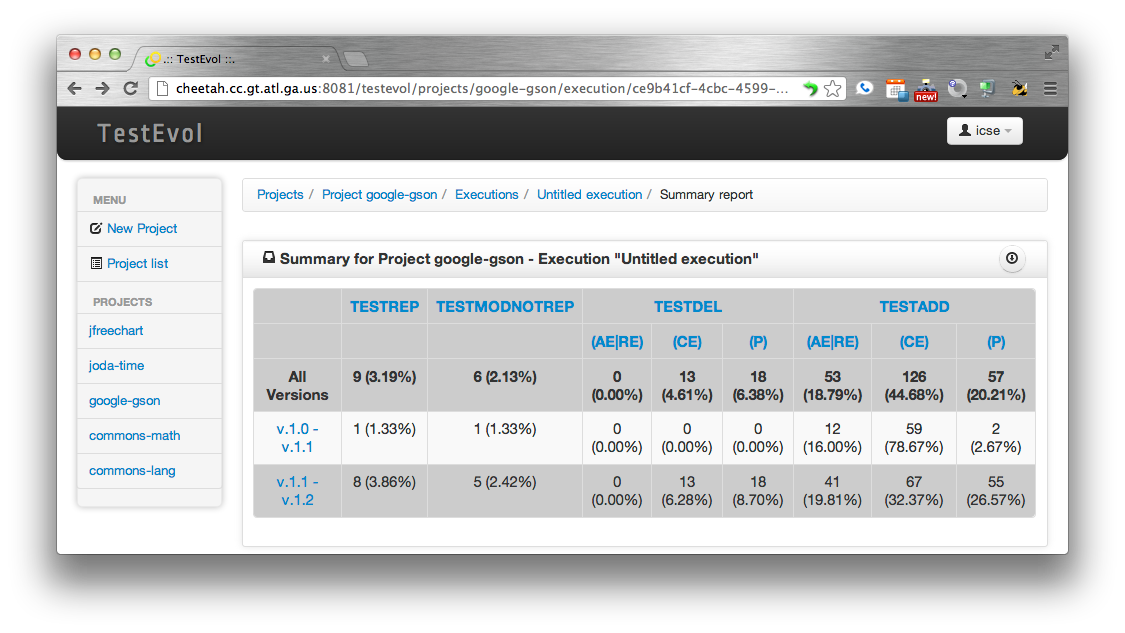
\includegraphics[width=\columnwidth]{1-summary}
        \vspace*{-20pt}
	\caption{Summary report for two pairs of versions of a
          project.}
        \vspace*{-8pt}
	\label{fig:summary}
\end{figure}

\begin{figure}[t]
	\centering
	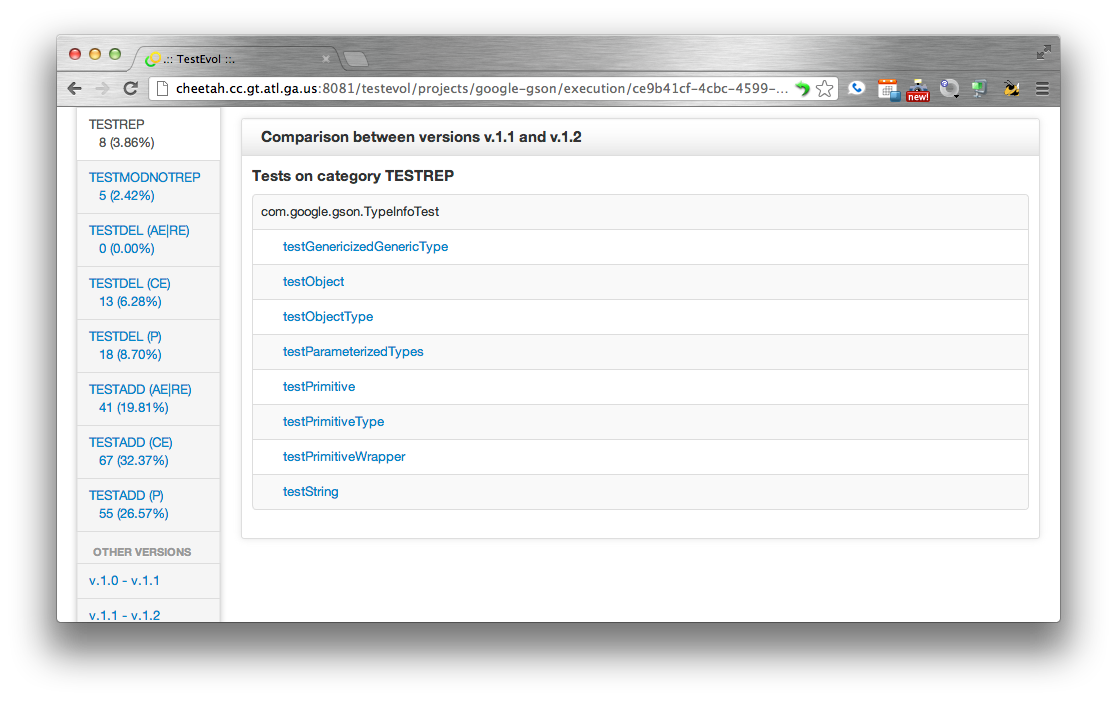
\includegraphics[width=\columnwidth]{2-versiondetails}
        \vspace*{-20pt}
	\caption{Detailed report for a pair of versions.}
        \vspace*{-8pt}
	\label{fig:versiondetails}
\end{figure}

\begin{figure}[t]
	\centering
	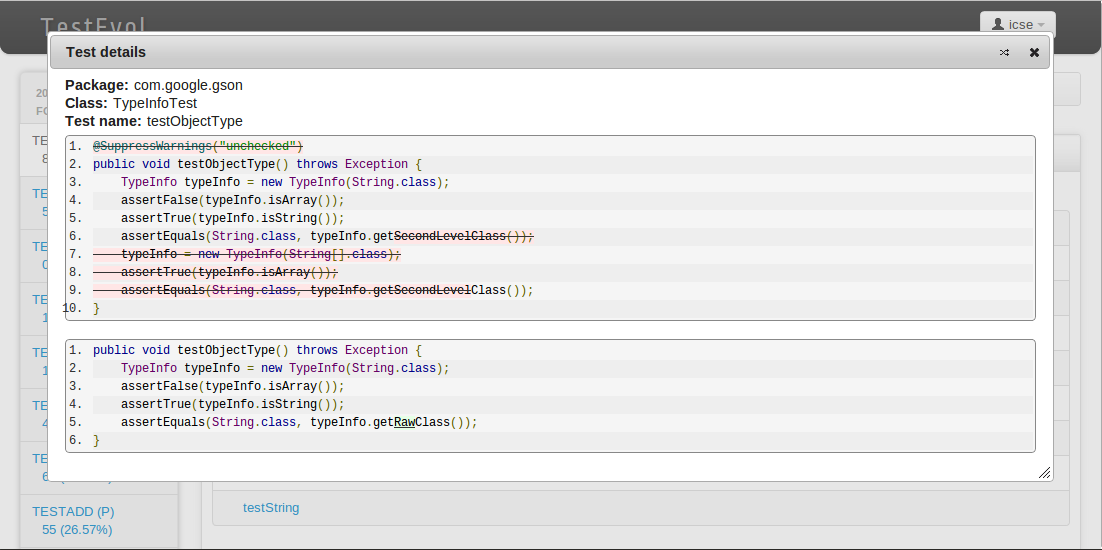
\includegraphics[width=\columnwidth]{3-testdetails}
        \vspace*{-20pt}
	\caption{Differences between two versions of a test case.}
        \vspace*{-8pt}
	\label{fig:testdetails}
\end{figure}

In terms of design, \tool\ consists of five components, as illustrated
in Figure~\ref{fig:trex}.
%
The \emph{compiler} component builds each system version and creates
two jar files, one containing the application classes and the other
containing the test classes.
%
The \emph{test-execution engine} analyzes each pair of system versions
$(S, S')$, where $S = (P, T)$ and $S' = (P', T')$.  First, it executes
$T$ on program $P$ and $T'$ on program $P'$ (\ie it runs the tests on
the respective program versions).  Then, it executes $T'$ on $P$ and
$T$ on $P'$. For each execution, it records the test outcome: $\pass,
\failce, \failae, or \failre$.
%
The \emph{differencing component} compares $T$ and $T'$ to identify
modified, deleted, and added tests. This component is implemented
using the \textsc{wala} analysis infrastructure for Java ({\small
  \url{wala.sourceforge.net}}).

The test outcomes, collected by the test-execution engine, and the
test-suite changes, computed by the differencing component, are then
passed to the \emph{test classifier}, which analyzes the information
about test outcomes and test updates to classify each update into one
of the eight test-evolution categories presented in
Section~\ref{sec:test-evolution}.  For each pair consisting of a
broken test case and its repaired version, the test classifier also
compares the test cases to identify the types of repair changes (\eg
different types of method-sequence changes and assertion changes), as
discussed in Section~\ref{sec:test-mod}. This analysis is also
implemented using \textsc{wala}.

\tool\ performs a further step for the test cases in categories
\catdelp{}and \cataddp{}. For these tests, the test classifier
leverages the \emph{coverage analyzer} to compute the branch coverage
achieved by each test; this facilitates the investigation of whether
the deleted or added tests cause any variations in the coverage
achieved by the new test suite.

\begin{figure}
	\centering
	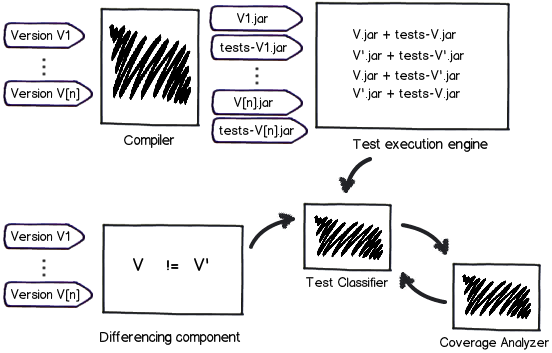
\includegraphics[width=\columnwidth]{architecture}
        \vspace*{-20pt}
	\caption{High-level design of \tool.}
        \vspace*{-8pt}
	\label{fig:trex}
\end{figure}

\vspace*{-8pt}
\section{Conclusion}
\label{sec:summary}

Test suites evolve throughout their lifetime and change together with
the applications under test. Adapting existing test cases manually,
however, can be extremely tedious, especially for large test suites,
which has motivated the recent development of automated test-repair
techniques. To support the development of more effective repair
techniques, and to help developers and testers better understand test
maintenance in general, we developed \tool. \tool is a tool for
systematic investigation of test-suite evolution that can provide its
users with a comprehensive understanding of how test cases evolve
throughout the lifetime of a software system. This demonstration
presents \tool, its main features, and its technical characteristics.
It also shows how \tool\ can be run on real-world software systems and
produce a wealth of useful information on how test-suite changes.

Complete information on \tool\ can be found on the tool's web page, at
{\small \url{http://www.cc.gatech.edu/~orso/software/testevol/}}.

% \section*{Acknowledgments}

% This work was supported in part by NSF awards CCF-0916605 and
% CCF-0964647 to Georgia Tech, and by funding from IBM Research and
% Microsoft Research.

\bibliographystyle{abbrv}
{\footnotesize
% \bibliography{paper}
\begin{thebibliography}{1}

\bibitem{Choudhary:2011}
S.~R. Choudhary, D.~Zhao, H.~Versee, and A.~Orso.
\newblock {WATER: Web Application TEst Repair}.
\newblock In {\em Proceedings of the First International Workshop on End-to-End
  Test Script Engineering}, pages 24--29, 2011.

\bibitem{Daniel:2010}
B.~Daniel, T.~Gvero, and D.~Marinov.
\newblock On test repair using symbolic execution.
\newblock In {\em Proceedings of the 19th International Symposium on Software
  Testing and Analysis}, pages 207--218, 2010.

\bibitem{Daniel:2009}
B.~Daniel, V.~Jagannath, D.~Dig, and D.~Marinov.
\newblock {ReAssert: Suggesting repairs for broken unit tests}.
\newblock In {\em Proceedings of the International Conference on Automated
  Software Engineering}, pages 433--444, 2009.

\bibitem{Grechanik:2009}
M.~Grechanik, Q.~Xie, and C.~Fu.
\newblock Maintaining and evolving gui-directed test scripts.
\newblock In {\em Proceedings of the 31st International Conference on Software
  Engineering}, pages 408--418, 2009.

\bibitem{Huang:2010}
S.~Huang, M.~B. Cohen, and A.~M. Memon.
\newblock Repairing {GUI} test suites using a genetic algorithm.
\newblock In {\em Proceedings of the 3rd International Conference on Software
  Testing, Verification and Validation}, pages 245--254, 2010.

\bibitem{Memon:2008}
A.~M. Memon.
\newblock {Automatically repairing event sequence-based GUI test suites for
  regression testing}.
\newblock {\em ACM Trans. Softw. Eng. Methodol.}, 18:1--36, November 2008.

\bibitem{Mirzaaghaei:2012}
M.~Mirzaaghaei, F.~Pastore, and M.~Pezz{\'e}.
\newblock Supporting test suite evolution through test case adaptation.
\newblock In {\em Proceedings of the 5th IEEE International Conference on
  Software Testing, Verification and Validation}, pages 231--240, 2012.

\bibitem{pinto12}
L.~S. Pinto, S.~Sinha, and A.~Orso.
\newblock Understanding myths and realities of test-suite evolution.
\newblock In {\em Proceedings of the 20th ACM SIGSOFT International Symposium
  on the Foundations of Software Engineering (FSE 2012), to appear}.

\end{thebibliography}

}

\end{document}

